%!TEX root = ../../book_ML.tex
% \chapter{Principal Component Analysis (phần 2/2)}

 
% Trong \href{http://machinelearningcoban.com/2017/06/15/pca/}{phần 1 của Principal Component Analysis} (PCA), một phương pháp giảm chiều dữ liệu rất quan trọng, chúng ta đã cùng ôn lại một vài kiến thức về Đại số tuyến tính và Thống kê, đồng thời, ý nghĩa toán học và các bước thực hiện PCA cũng đã được trình bày. Trong phần 2 này, chúng ta cùng tìm hiểu thêm một vài tính chất quan trọng của PCA cũng như các ứng dụng nổi bật của PCA trong các bài toán Machine Learning. 
 
% \textit{Các bạn được khuyến khích đọc \href{http://machinelearningcoban.com/2017/06/07/svd/}{Bài 26} và \href{http://machinelearningcoban.com/2017/06/15/pca/}{Bài 27} trước khi đọc bài này.} 
 
 
\section{Mối quan hệ giữa PCA và SVD}
Giữa PCA và SVD có mỗi quan hệ đặc biệt với nhau. Để nhận ra điều này, tôi xin được nhắc lại hai điểm đã trình bày sau đây: 
 
 
\subsection{SVD cho bài toán xấp xỉ low-rank tốt nhất}
Nghiệm $\mathbf{A}$ của bài toán xấp xỉ một ma trận bởi một ma trận khác có rank không vượt quá $k$: 
\begin{equation} 
\label{eqn:28_1}
\begin{aligned} 
  \min_{\mathbf{A}} &\|\mathbf{X} - \mathbf{A}\|_F \\\ 
  \text{s.t.} & \text{rank}(\mathbf{A}) = K 
\end{aligned} 
\end{equation} 
 
chính là \href{http://machinelearningcoban.com/2017/06/07/svd/#-truncated-svd}{Truncated SVD} của $\mathbf{A}$. Cụ thể, nếu SVD của $\mathbf{X} \in\mathbb{R}^{D\times N}$ là: 
\begin{equation} 
  \mathbf{X} = \mathbf{U}\mathbf{\Sigma}\mathbf{V}^T 
\end{equation} 
với $\mathbf{U} \in \mathbb{R}^{D \times D}$ và $\mathbf{V}\in \mathbb{R}^{N\times N}$ là các ma trận trực giao, và $\mathbf{\Sigma} \in \mathbb{R}^{D \times N}$ là ma trận đường chéo (không nhất thiết vuông) với các phần tử trên đường chéo không âm giảm dần, thì nghiệm của bài toán \eqref{eqn:28_1} chính là: 
\begin{equation} 
  \label{eqn:28_2}
  \mathbf{A} = \mathbf{U}_K \mathbf{\Sigma}_K \mathbf{V}_K^T
\end{equation} 
 
với $\mathbf{U} \in \mathbb{R}^{D \times K}$ và $\mathbf{V}\in \mathbb{R}^{N\times K}$ là các ma trận tạo bởi $K$ cột đầu tiên của $\mathbf{U}$ và $\mathbf{V}$, và $\mathbf{\Sigma}_K \in \mathbb{R}^{K \times K}$ là ma trận đường chéo con ứng với $K$ hàng đầu tiên và $K$ cột đầu tiên của $\mathbf{\Sigma}$. 
 
 
\subsection{Ý tưởng của PCA}
Trong PCA, như đã chứng minh ở \eqref{eqn:27_10}, PCA là bài toán đi tìm ma trận trực giao $\mathbf{U}$ và ma trận mô tả dữ liệu ở không gian thấp chiều $\mathbf{Z}$ sao cho việc xấp xỉ sau đây là tốt nhất: 
\begin{equation} 
\label{eqn:28_3}
\mathbf{X} \approx \tilde{\mathbf{X}} = \mathbf{U}_K \mathbf{Z} + \bar{\mathbf{U}}_K \bar{\mathbf{U}}_K^T\bar{\mathbf{x}}\mathbf{1}^T 
\end{equation} 
với $\mathbf{U}_K, \bar{\mathbf{U}}_K$ lần lượt là các ma trận được tạo bởi $K$ cột đầu tiên và $D-K$ cột cuối cùng của ma trận trực giao $\mathbf{U}$, và $\bar{\mathbf{x}}$ là vector kỳ vọng của dữ liệu. 
 
\textbf{Giả sử rằng vector kỳ vọng $\bar{\mathbf{x}} = \mathbf{0}$}. Khi đó, \eqref{eqn:28_3} tương đương với: 
\begin{equation} 
\label{eqn:28_4}
\mathbf{X} \approx \tilde{\mathbf{X}} = \mathbf{U}_K \mathbf{Z}
\end{equation} 
 
Bài toán tối ưu của PCA sẽ trở thành: 
\begin{equation} 
\label{eqn:28_5}
\begin{aligned} 
  \mathbf{U}_K, \mathbf{Z} &=& \min_{\mathbf{U}_K, \mathbf{Z} } \|\mathbf{X} - \mathbf{U}_K \mathbf{Z}\|_F\\\ 
  \text{s.t.:}&& \mathbf{U}_K^T \mathbf{U}_K = \mathbf{I}_K & 
\end{aligned} 
\end{equation} 
với $\mathbf{I}_K \in \mathbb{R}^{K\times K}$ là ma trận đơn vị trong không gian $K$ chiều, và điều kiện ràng buộc là để đảm bảo các cột của $\mathbf{U}_K$ tạo thành một hệ trực chuẩn. 
 
 
\subsection{Quan hệ giữa PCA và SVD}
Bạn có nhận ra điểm tương đồng giữa hai bài toán tối ưu \eqref{eqn:28_1} và \eqref{eqn:28_5} với nghiệm của bài toán đầu tiên được cho trong \eqref{eqn:28_2}? Bạn có thể nhận ra ngay nghiệm của bài toán \eqref{eqn:28_5} chính là: 
\begin{eqnarray} 
  \mathbf{U}_K \quad \text{in}\quad (5) &=& \mathbf{U}_K\quad \text{in} \quad \eqref{eqn:28_2} \\\ 
  \mathbf{Z} \quad\text{in}\quad (5) &=& \mathbf{\Sigma}_K \mathbf{V}_K^T \quad \text{in} \quad \eqref{eqn:28_2} 
\end{eqnarray} 
 
Như vậy, nếu các điểm dữ liệu được biễu diễn bởi các cột của một ma trận, và trung bình cộng của mỗi hàng của ma trận đó bằng 0 (để cho vector kỳ vọng bằng 0), thì nghiệm của bài toán PCA được rút ra trực tiếp từ Truncated SVD của ma trận đó. Nói cách khác, nghiệm của PCA chính là một trường hợp đặc biệt của bài toán Matrix Factorization giải bằng SVD. 
 
 
\section{Làm thế nào để chọn chiều của dữ liệu mới}
 
Một câu hỏi được đặt ra là, làm thế nào để chọn ra giá trị $K$ - chiều của dữ liệu mới - với từng loại dữ liệu khác nhau? 
 
Có một cách xác định $K$ là dựa trên việc \textit{lượng thông tin muốn giữ lại}. Như đã trình bày, PCA còn được gọi là phương pháp tối đa \textit{tổng phương sai được giữ lại}. Vậy ta có thể coi tổng các phương sai được giữ lại là lượng thông tin được giữ lại. Với phương sai càng lớn, tức dữ liệu có độ phân tán cao, thể hiện lượng thông tin càng lớn. 
 
 Nhắc lại rằng trong mọi hệ trục toạ độ, tổng phương sai của dữ liệu là như nhau và bằng tổng các trị riêng của ma trận hiệp phương sai $\sum_{i=1}^D \lambda_i$. Thêm nữa, PCA giúp giữ lại lượng thông tin (tổng các phương sai) là: $\sum_{i=1}^K \lambda_i$. Vậy ta có thể coi biểu thức: 
\begin{equation} 
 \label{eqn:28_6}
   r_K = \frac{\sum_{i=1}^K \lambda_i}{\sum_{j=1}^D \lambda_j} 
\end{equation} 
là lượng thông tin được giữ lại khi số chiều dữ liệu mới sau PCA là $K$. 
 
Như vậy, giả sử ta muốn giữ lại 99\% dữ liệu, ta chỉ cần chọn $K$ là số tự nhiên nhỏ nhất sao cho $r_K \geq 0.99$. 
 
Khi dữ liệu phân bố quanh một không gian con, các giá trị phương sai lớn nhất ứng với các $\lambda_i$ đầu tiên lớn hơn nhiều so với các phương sai còn lại. Khi đó, ta có thể chọn được $K$ khá nhỏ để đạt được $r_K \geq 0.99$. 
 
 
\section{Lưu ý về tính PCA trong các bài toán thực tế}
Có hai trường hợp trong thực tế mà chúng ta cần lưu ý về PCA. Trường hợp thứ nhất là lượng dữ liệu có được nhỏ hơn rất nhiều so với số chiều dữ liệu. Trường hợp thứ hai là khi lượng dữ liệu trong tập training là rất lớn, có thể lên tới cả triệu. Việc tính toán ma trận hiệp phương sai và trị riêng đôi khi trở nên bất khả thi. Có những hướng giải quyết hiệu quả cho các trường hợp này. 
 
\textbf{Trong mục này, ta sẽ coi như dữ liệu đã được chuẩn hoá, tức đã được trừ đi vector kỳ vọng. Khi đó, ma trận hiệp phương sai sẽ là $\mathbf{S} = \frac{1}{N}\mathbf{X}\mathbf{X}^T$.} 
 
\subsection{Số chiều dữ liệu nhiều hơn số điểm dữ liệu}
 
Đó là trường hợp $D > N$, tức ma trận dữ liệu $\mathbf{X}$ là một 'ma trận cao'. Khi đó, số trị riêng khác không của ma trận hiệp phương sai $\mathbf{S}$ sẽ không vượt quá rank của nó, tức không vượt quá $N$. Vậy ta cần chọn $K < N$ vì không thể chọn ra được $N$ trị riêng khác 0 của một ma trận có rank bằng $N$. 
 
Việc tính toán các trị riêng và vector riêng cũng có thể được thực hiện một cách hiệu quả dựa trên các tính chất sau đây: 

\textbf{Tính chất 1:} Trị riêng của $\mathbf{A}$ cũng là trị riêng của $k\mathbf{A}$ với $k \neq 0$ bất kỳ. Điều này có thể được suy ra trực tiếp từ định nghĩa của trị riêng và vector riêng. 
 
\textbf{Tính chât 2:} Trị riêng của $\mathbf{AB}$ cũng là trị riêng của $\mathbf{BA}$ với $\mathbf{A} \in \mathbb{R}^{d_1 \times d_2}, \mathbf{B} \in \mathbb{R} ^{d_2 \times d_1}$ là các ma trận bất kỳ và $d_1, d_2$ là các số tự nhiên khác không bất kỳ. Tôi xin không chứng minh quan sát này. 
 
Như vậy, thay vì tìm trị riêng của ma trận hiệp phương sai $\mathbf{S} \in \mathbb{R}^{D\times D}$, ta đi tìm trị riêng của ma trận $\mathbf{T} = \mathbf{X}^T \mathbf{X} \in \mathbb{R}^{N \times N}$ có số chiều nhỏ hơn (vì $N < D$). 
 
\textbf{Tính chất 3:} Giả sử $(\lambda, \mathbf{u})$ là một cặp trị riêng - vector riêng của $\mathbf{T}$, thế thì $(\lambda, \mathbf{Xu})$ là một cặp trị riêng - vector riêng của $\mathbf{S}$. 
 
Thật vậy: 
\begin{eqnarray} 
  \label{eqn:28_7}
  \mathbf{X}^T \mathbf{Xu} &=& \lambda \mathbf{u} \\\ 
  \label{eqn:28_8}
  \Rightarrow (\mathbf{X}\mathbf{X}^T)(\mathbf{Xu}) &=& \lambda \mathbf{Xu}  
\end{eqnarray} 
 
Biểu thức \eqref{eqn:28_7} là theo định nghĩa của trị riêng và vector riêng. Biểu thức \eqref{eqn:28_8} thu được từ \eqref{eqn:28_7} bằng cách nhân bên trái cả hai vế với ma trận $\mathbf{X}$. Từ \eqref{eqn:28_8} ta suy ra \textbf{Quan sát 3}. 
 
Như vậy, ta có thể hoàn toàn tính được trị riêng và vector riêng của ma trận hiệp phương sai dựa trên một ma trận nhỏ hơn. 
 
 
\subsubsection{Chuẩn hoá các vector riêng}
 
\textit{Nhắc lại định nghĩa không gian riêng: Không gian riêng ứng với trị riêng của một ma trận là không gian sinh (span subspace) tạo bởi toàn bộ các vector riêng ứng với trị riêng đó.} 
 
Việc cuối cùng phải làm là chuẩn hoá các vector riêng tìm được sao cho chúng tạo thành một hệ trực chuẩn. Việc này có thể dựa trên hai điểm sau đây: 
 
\textbf{Thứ nhất}, nếu $\mathbf{A}$ là một ma trận đối xứng, $(\lambda_1, \mathbf{x}_1), (\lambda_2, \mathbf{x}_2)$ là các căp trị riêng - vector riêng của $\mathbf{A}$ với $\lambda_1 \neq \lambda_2$, thế thì $\mathbf{x}_1^T\mathbf{x}_2 = 0$. Nói cách khác, hai vector bất kỳ trong hai không gian riêng khác nhau của một ma trận đối xứng thì trực giao với nhau. Chứng minh cho tính chất này có thể được thấy trong một dòng dưới đây: 
\begin{eqnarray} 
  \mathbf{x}_2^T \mathbf{Ax}_1 = \mathbf{x}_1^T \mathbf{Ax}_2 = \lambda_1 \mathbf{x}_2^T \mathbf{x}_1 = \lambda_2 \mathbf{x}_1^T \mathbf{x}_2 \Rightarrow \mathbf{x}_1^T \mathbf{x}_2 = 0 
\end{eqnarray} 
Dấu bằng cuối cùng xảy ra vì $\lambda_1 \neq \lambda_2$. 
 
\textbf{Thứ hai}, với các trị riêng độc lập tìm được trong một không gian riêng, ta có thể dùng Gram-Schmit process để chuẩn hoá chúng về một hệ trực chuẩn. 
 
Kết hợp hai điểm trên, ta có thể thu được các vector riêng tạo thành một hệ trực chuẩn, chính là ma trận $\mathbf{U}_K$ trong PCA. 
 
 
\subsection{Với các bài toán large-scale}
Trong rất nhiều bài toán, cả $D$ và $N$ đều là các số rất lớn, đồng nghĩa với việc ta phải tìm trị riêng cho một ma trận rất lớn. Ví dụ, có 1 triệu bức ảnh 1000 $\times$ 1000 pixel, như vậy $D = N = 10^6$ là một số rất lớn, việc trực tiếp tính toán trị riêng và vector riêng cho ma trận hiệp phương sai là không khả thi. Tuy nhiên, có một phương pháp cho phép tính xấp xỉ các giá trị này một cách nhanh hơn. Phương pháp đó có tên là \href{http://www.cs.huji.ac.il/~csip/tirgul2.pdf}{Power Method}. 
 
Phương pháp này nói rằng, nếu thực hiện quy trình sau, ta sẽ tìm được cặp trị riêng và vector đầu tiên của một ma trận nửa xác định dương: 
% <hr> 
\textbf{Phương pháp Power tìm trị riêng và vector riêng của một ma trận nửa xác định dương $\mathbf{A} \in \mathbb{R}^{n \times n}$}: 
\begin{enumerate}
  \item Chọn một vector $\mathbf{q}^{(0)} \in \mathbb{R}^n, \|\mathbf{q}^{(0)}\|_2 = 1$ bất kỳ. 
  \item Với $k = 1, 2, \dots$, tính: $\mathbf{z} = \mathbf{Aq}^{(k-1)}$. 
  \item Chuẩn hoá: $\mathbf{q}^{(k)} = \mathbf{z} / \|\mathbf{z}\|_2$. 
  \item Nếu $\|\mathbf{q}^{(k)} - \mathbf{q}^{(k-1)}\|_2$ đủ nhỏ thì dừng lại. Nếu không, $k := k + 1$ rồi quay lại Bước 2. 
  \item $\mathbf{q}^{(k)}$ chính là vector riêng ứng với trị riêng lớn nhất $\lambda_1 = (\mathbf{q}^{(k)})^T\mathbf{A}\mathbf{q}^{(k)}$. 
\end{enumerate}
% <hr> 
 
Quy trình này hội tụ khá nhanh và đã được chứng minh \href{http://www.cs.huji.ac.il/~csip/tirgul2.pdf}{tại đây}. Phần chứng minh tương đối đơn giản và không mang lại nhiều thông tin hữu ích, tôi xin được bỏ qua. 
 
Để tìm vector riêng và trị riêng thứ hai của ma trận $\mathbf{A}$, chúng ta dựa trên định lý sau: 

\textbf{Định lý:} Nếu ma trận nửa xác định dương $\mathbf{A}$ có các trị riêng $\lambda_1 \geq \lambda_2 \geq \dots \geq \lambda_n ( \geq 0)$ và các vector riêng tương ứng $\mathbf{v}_1, \dots, \mathbf{v}_n$, hơn nữa các vector riêng này tạo thành 1 hệ trực chuẩn, thì ma trận: 
\begin{equation} 
  \mathbf{B} = \mathbf{A} - \lambda_1 \mathbf{v}_1 \mathbf{v}_1^T 
\end{equation} 
có các trị riêng $\lambda_2 \geq \lambda_3 \geq \dots \geq \lambda_n \geq 0$ và các vector riêng tương ứng là $\mathbf{v}_2, \mathbf{v}_3, \dots, \mathbf{v}_n, \mathbf{v}_1$. 

\textit{Chứng minh: }
 
Với $i = 1$: 
\begin{eqnarray} 
  \mathbf{Bv}_1 &=& (\mathbf{A} - \lambda_1 \mathbf{v}_1 \mathbf{v}_1^T) \mathbf{v} \\\
  &= & \mathbf{Av}_1 - \lambda_1 \mathbf{v}_1 = \mathbf{0} \\\ 
\end{eqnarray} 
 
Với $i > 1$: 
\begin{eqnarray} 
  \mathbf{Bv}_i &=& (\mathbf{A} - \lambda_1 \mathbf{v}_1 \mathbf{v}_1^T)\mathbf{v}_i \\\ 
  &=& \mathbf{Av}_i - \lambda_1 \mathbf{v}_1 (\mathbf{v}_1^T \mathbf{v}_i) \\\ 
  &=& \mathbf{Av}_i = \lambda_i \mathbf{v}_i 
\end{eqnarray} 
 
Như vậy định lý đã được chứng minh $\square$. 
 
Lúc này, $(\lambda_2, \mathbf{v}_2)$ lại trở thành cặp trị riêng-vector riêng lớn nhất của $\mathbf{B}$. Cách tìm hai biến số này một lần nữa được thực hiện bằng Phương pháp Power. 
 
Tiếp tục quy trình này, ta sẽ tìm được (xấp xỉ) tất cả các trị riêng và vector riêng tương ứng của ma trận hiệp phương sai. Cũng xin lưu ý rằng ta chỉ cần tìm tới trị riêng thứ $K$ của ma trận hiệp phương sai. Cách làm này trên thực tế được sử dụng rất nhiều. 
 
Phương pháp Power còn là thuật toán cơ bản trong \href{https://en.wikipedia.org/wiki/PageRank}{Google PageRank} giúp sắp xếp các website theo mức độ phổ biến giảm dần. PageRank chính là nền móng của Google; ngày nay, việc tìm kiếm trong Google sử dụng nhiều thuật toán nâng cao hơn PageRank. Tôi sẽ có một bài riêng về Google PageRank sau khi nói về Chuỗi Markov và Mô hình Markov ẩn. 
 
 
\section{Ví dụ trên Python}
 
 
\subsection{Eigenface}
\href{https://en.wikipedia.org/wiki/Eigenface}{Eigenface} là một trong các phương pháp phổ biến nhất trong bài toán nhận dạng khuôn mặt. Ý tưởng của Eigenface là đi tìm một không gian có số chiều nhỏ hơn để mô tả mỗi khuôn mặt, từ đó sử dụng vector trong không gian thấp này như là feature vector cho việc thực hiện classification. Điều đáng nói là một bức ảnh khuôn mặt có kích thước khoảng 200 $\times$ 200 sẽ có số chiều là 40k - là một số cực lớn, trong khi đó, feature vector thường chỉ có số chiều bằng vài trăm. 
 
Eigenface thực ra chính là PCA. Các Eigenfaces chính là các eigenvectors ứng với các trị riêng lớn nhất của ma trận hiệp phương sai. 
 
Trong phần này, chúng ta cùng làm một thí nghiệm nhỏ trên cơ sở dữ liệu \href{http://vismod.media.mit.edu/vismod/classes/mas622-00/datasets/}{Yale face database}. Các bức ảnh trong thí nghiệm này đã được căn chỉnh cho cùng với kích thước và khuôn mặt nằm trọn vẹn trong một hình chữ nhật có kích thước $116 \times  98$ pixel. Có tất cả 15 người khác nhau, mỗi người có 11 bức ảnh được chụp ở các điều kiện ánh sáng và cảm xúc khác nhau, bao gồm: 'centerlight', 'glasses', 'happy', 'leftlight', 'noglasses', 'normal', 'rightlight','sad', 'sleepy', 'surprised', và 'wink'. 
 
Hình \ref{fig:28_1} minh hoạ ví dụ về các bức ảnh của người có id là 10. 
% <hr> 
% <div class="imgcap"> 
% <img src ="/assets/28_pca2/yaleb_exs.png" align = "center" width = "800"> 
% </div> 
 
% <div class = "thecap" align = "left">Hình 1: Ví dụ về ảnh của một người trong Yale Face Database. </div> 
% <hr> 

\begin{figure}[t]
\centering
    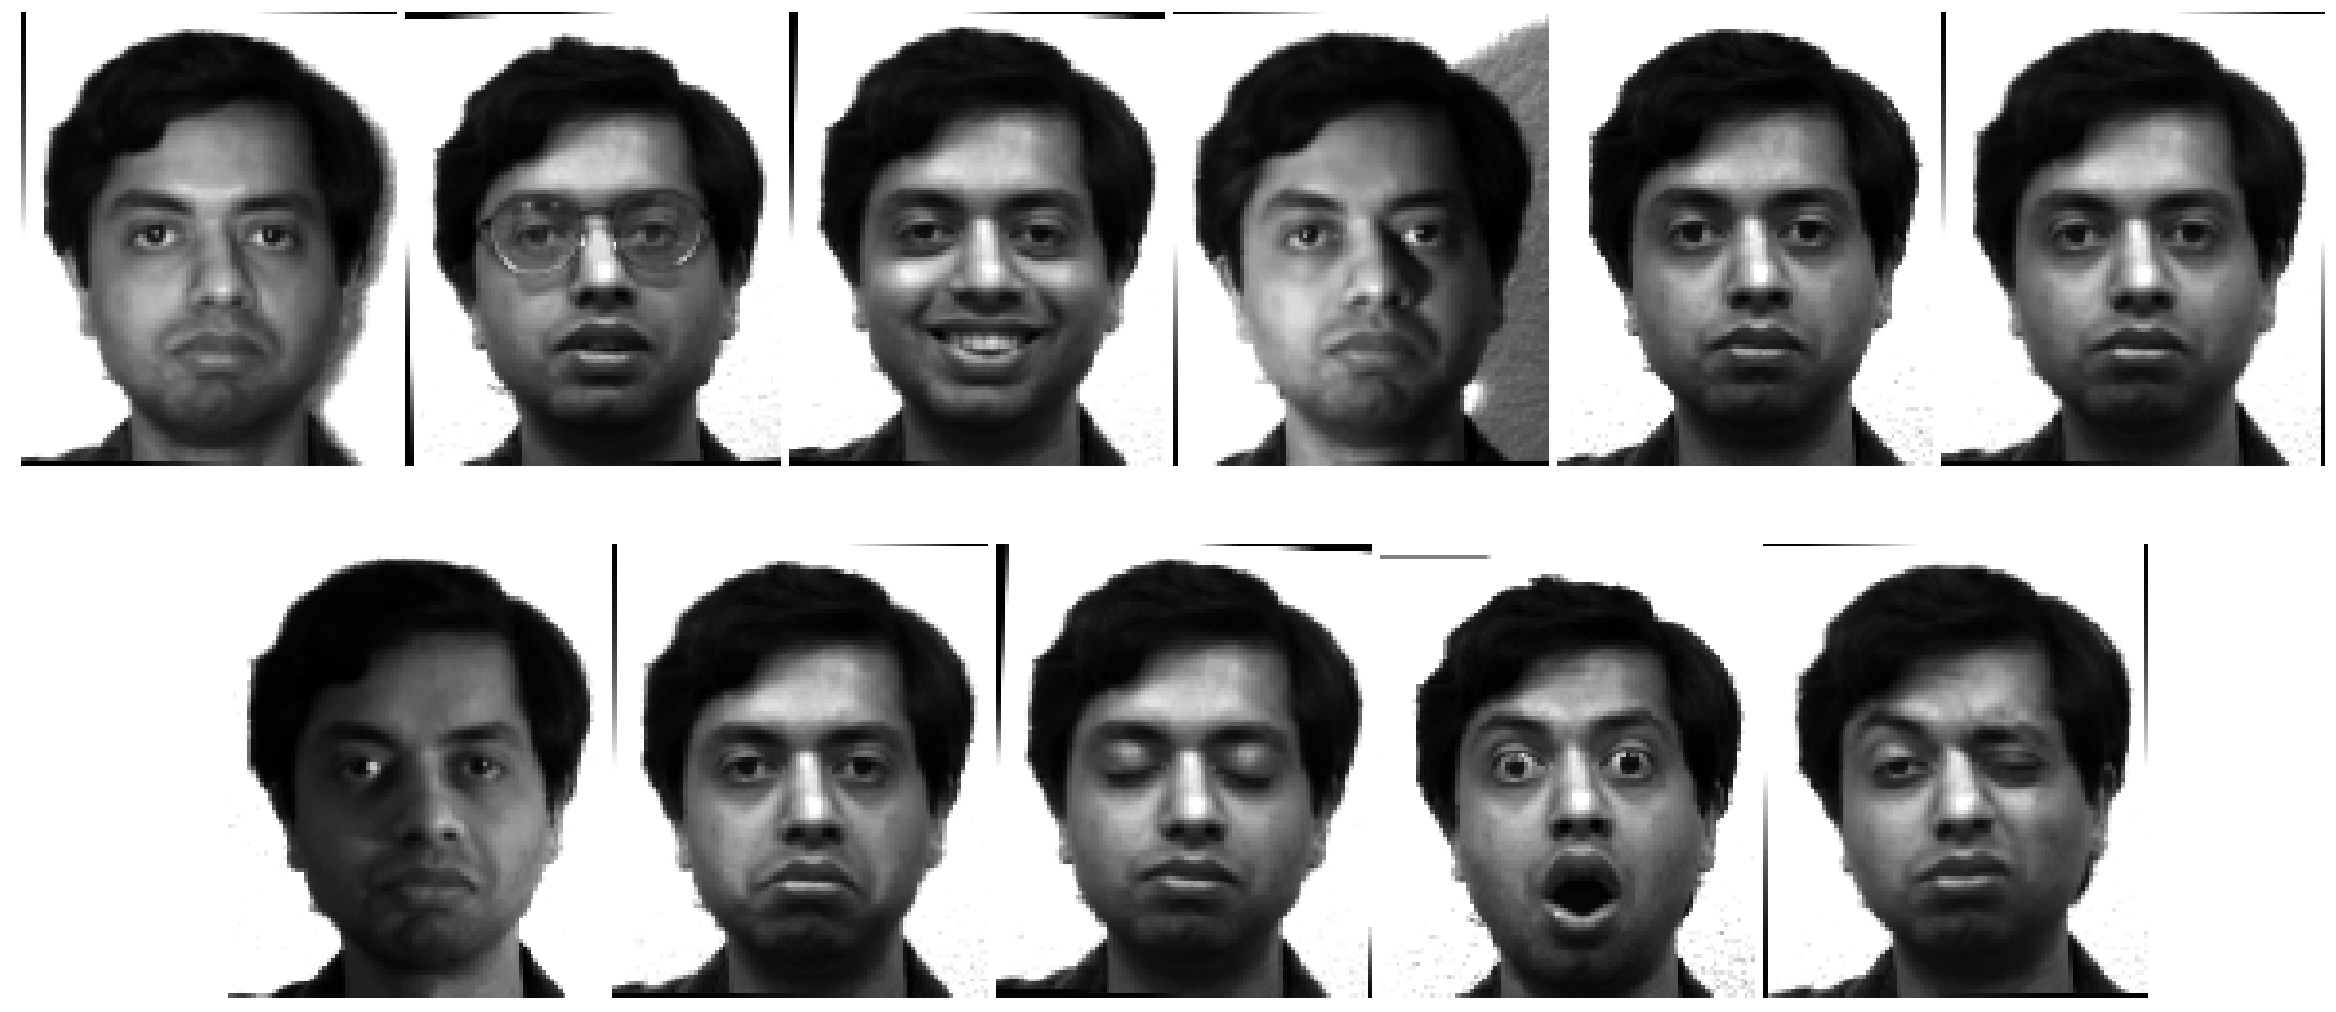
\includegraphics[width = \textwidth]{Chapters/07_DimemsionalityReduction/28_pca2/latex/yaleb_exs.pdf}
    \caption[]{Ví dụ về ảnh của một người trong Yale Face Database.}
    \label{fig:28_1}
\end{figure}
Ta có thể thấy rằng số chiều dữ liệu là $116 \times 98 = 11368$ là một số khá lớn. Tuy nhiên, vì chỉ có tổng cộng $15 \times 11 = 165$ bức ảnh nên ta có thể nén các bức ảnh này về dữ liệu mới có chiều nhỏ hơn 165. Trong ví dụ này, tôi chọn $K = 100$. 
 
Dưới đây là đoạn code thực hiện PCA cho toàn bộ dữ liệu. Chú ý rằng tôi sử dụng thư viện \pythoninline{sklearn}. 
 
\begin{lstlisting}[language=Python]
import numpy as np 
from scipy import misc                     # for loading image 
np.random.seed(1) 
 
# filename structure 
path = 'unpadded/' # path to the database 
ids = range(1, 16) # 15 persons 
states = ['centerlight', 'glasses', 'happy', 'leftlight', 
          'noglasses', 'normal', 'rightlight','sad', 
          'sleepy', 'surprised', 'wink' ] 
prefix = 'subject' 
surfix = '.pgm' 
 
# data dimension 
h = 116 # hight 
w = 98 # width 
D = h * w 
N = len(states)*15 
K = 100 
 
# collect all data 
X = np.zeros((D, N)) 
cnt = 0 
for person_id in range(1, 16): 
    for state in states: 
        fn = path + prefix + str(person_id).zfill(2) + '.' + state + surfix 
        X[:, cnt] = misc.imread(fn).reshape(D) 
        cnt += 1 
 
# Doing PCA, note that each row is a datapoint 
from sklearn.decomposition import PCA 
pca = PCA(n_components=K) # K = 100 
pca.fit(X.T) 
 
# projection matrix 
U = pca.components_.T 
\end{lstlisting}
 
Chú ý rằng các hàm của \pythoninline{sklearn} đều chọn dữ liệu ở dạng hàng. Còn tôi thường chọn dữ liệu ở dạng cột cho thuận tiện trong biểu diễn toán học. Trước khi sử dụng \pythoninline{sklearn}, bạn đọc chú ý chuyển vị ma trận dữ liệu. 
 
Trong dòng \pythoninline{pca = PCA(n_components=K)}, nếu \pythoninline{n_components} là một số thực trong khoảng $(0, 1)$, PCA sẽ thực hiện việc tìm $K$ dựa trên biểu thức $(6)$. 
 
Hình \ref{fig:28_2} biểu diễn 18 vector riêng đầu tiên tìm được bằng PCA. Các vector tìm được ở dạng vector cột, ta cần phải \pythoninline{reshape} chúng để có thể minh hoạ như các bức ảnh. 
 
% <hr> 
% <div class="imgcap"> 
% <img src ="/assets/28_pca2/yaleb_eig.png" align = "center" width = "800"> 
% </div> 
 
% <div class = "thecap" align = "left">Hình 2: Các eigenfaces tìm được bằng PCA. </div> 
% <hr> 

\begin{figure}[t]
\centering
    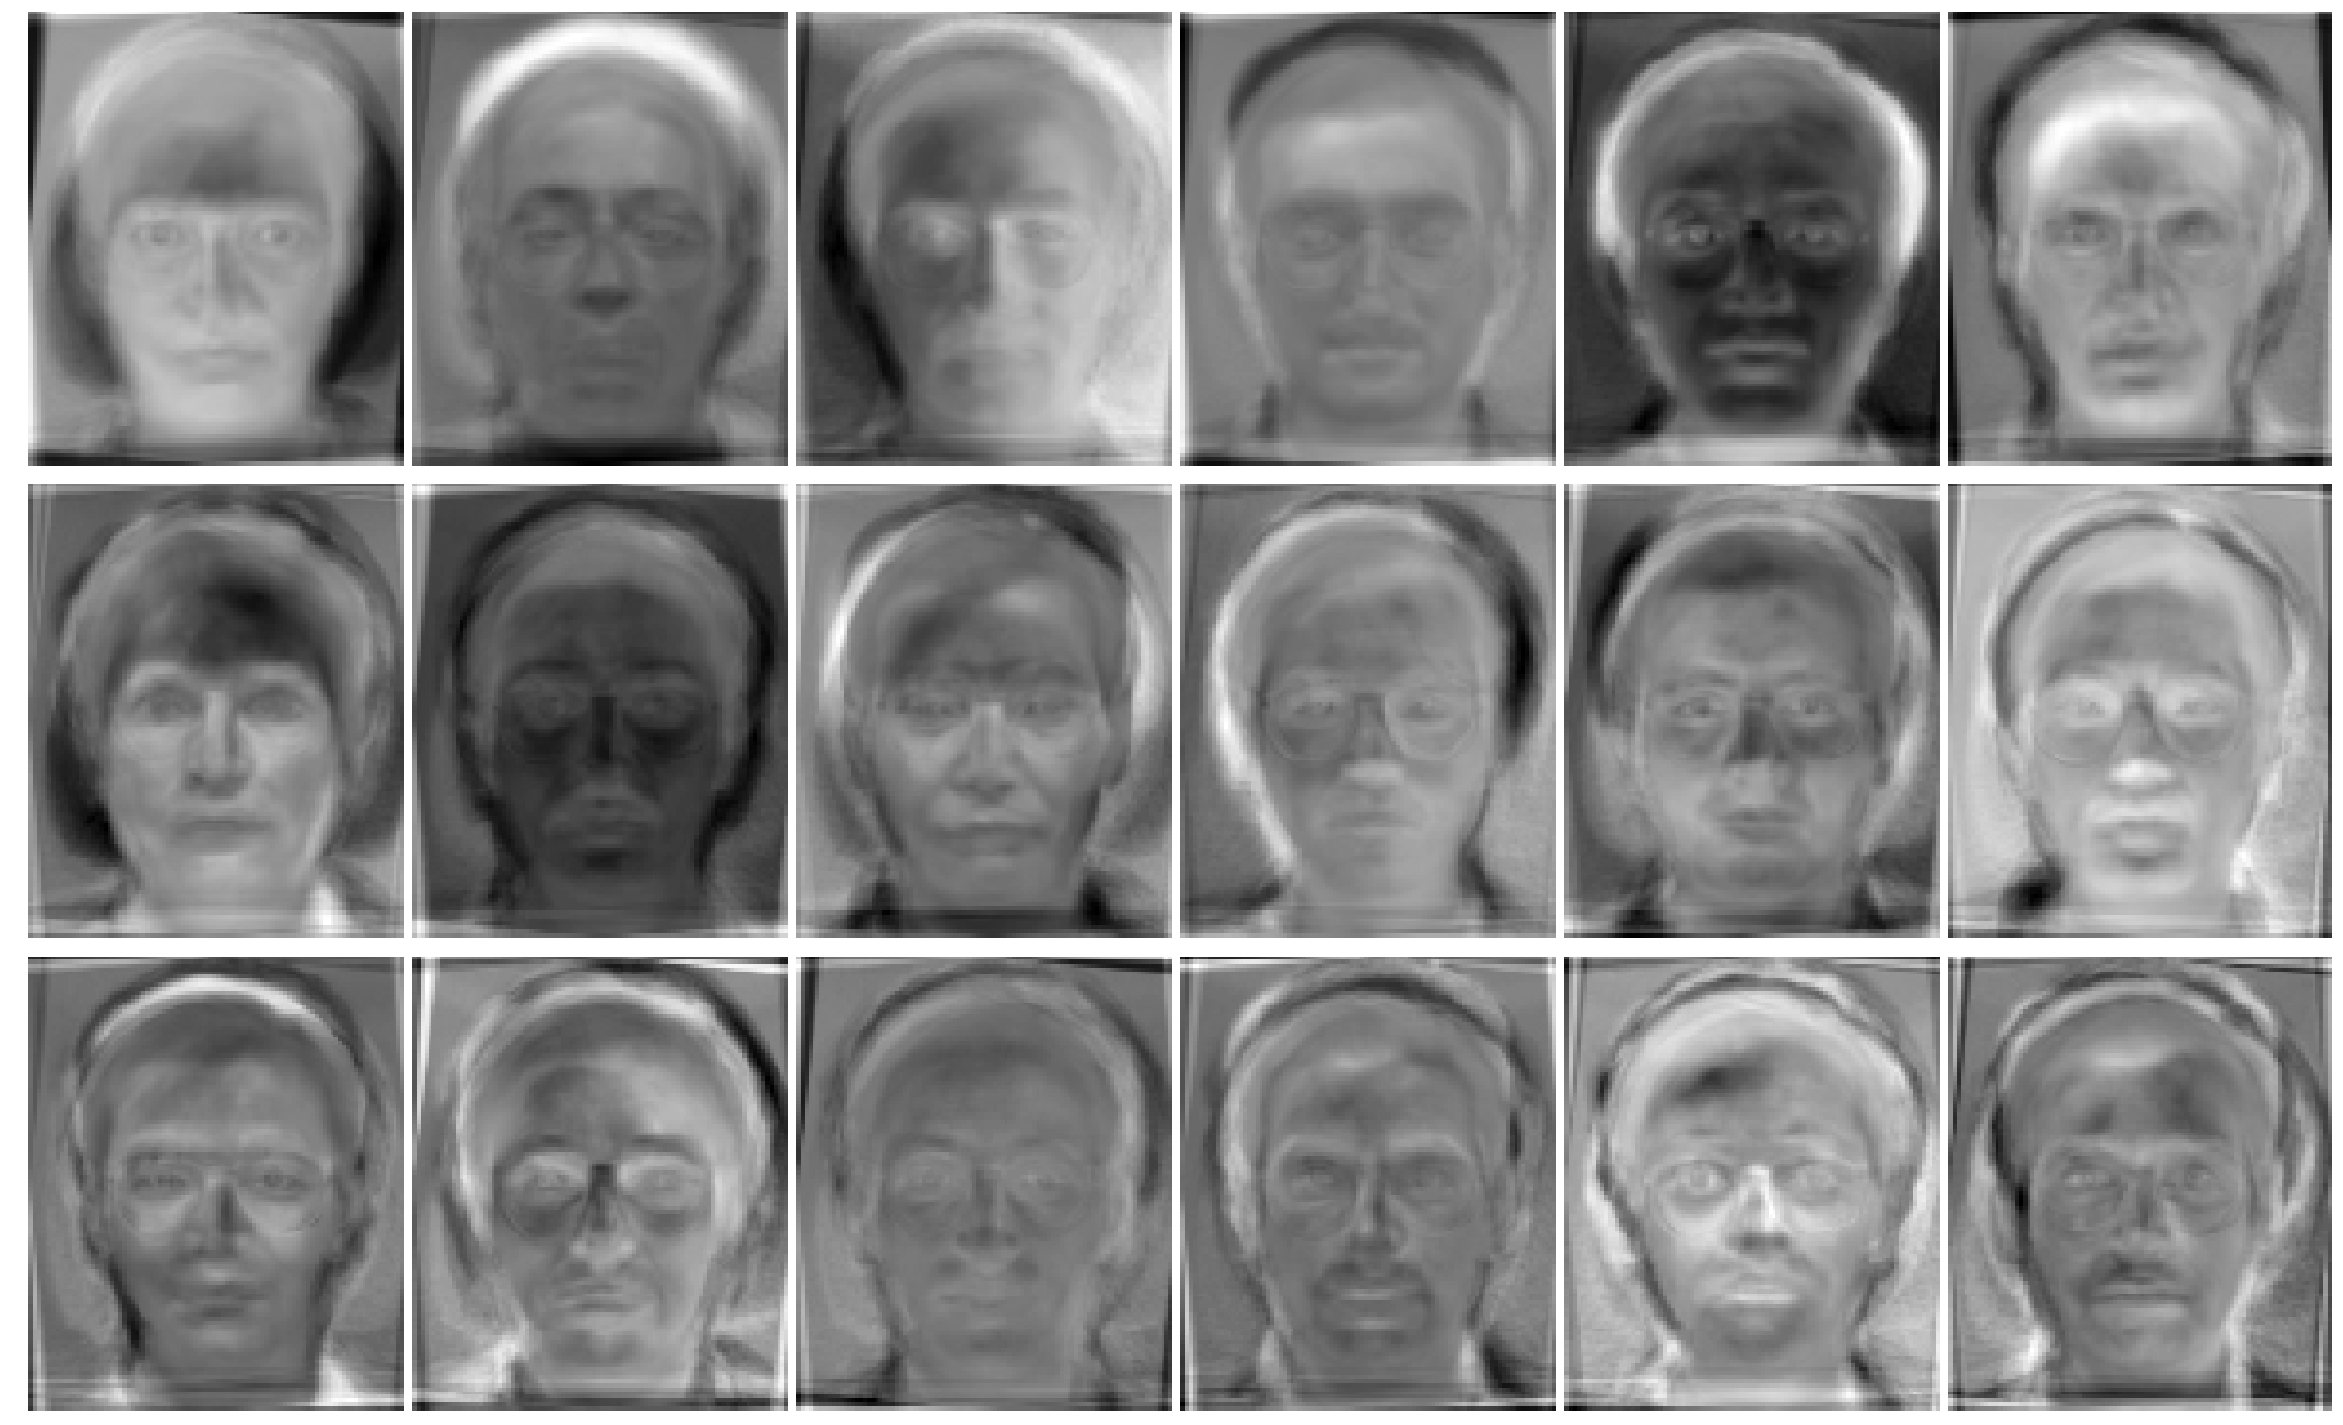
\includegraphics[width = \textwidth]{Chapters/07_DimemsionalityReduction/28_pca2/latex/yaleb_eig.pdf}
    \caption[]{Các eigenfaces tìm được bằng PCA.}
    \label{fig:28_2}
\end{figure}
 
Có một điều dễ nhận ra là các ảnh minh hoạ các vector thu được ít nhiều mang thông tin của mặt người. Thực tế, một khuôn mặt gốc sẽ được xấp xỉ như tổng có trọng số của các \textit{khuôn mặt} này. Vì các vector riêng này đóng vai trò như cơ sở của không gian mới với ít chiều hơn, chúng còn được gọi là \textit{khuôn mặt riêng}, tức \textit{eigenfaces}. 
 
Để xem mức độ hiệu quả của Eigenfaces như thế nào, chúng ta thử minh hoạ các bức ảnh gốc và các bức ảnh được xấp xỉ bằng PCA, kết quả được cho như Hình 3 dưới đây: 
% <hr> 
% <div class="imgcap"> 
% <img src ="/assets/28_pca2/yaleb_ori_res.png" align = "center" width = "800"> 
% </div> 
 

% <div class = "thecap" align = "left">Hình 3: Hàng trên: các ảnh gốc. Hàng dưới: các ảnh được \textit{suy ra} từ eigenfaces. Ảnh ở hàng dưới có nhiều nhiễu nhưng vẫn mang những đặc điểm riêng mà mắt người có thể phân biệt được. </div> 
% <hr> 
\begin{figure}[t]
\centering
    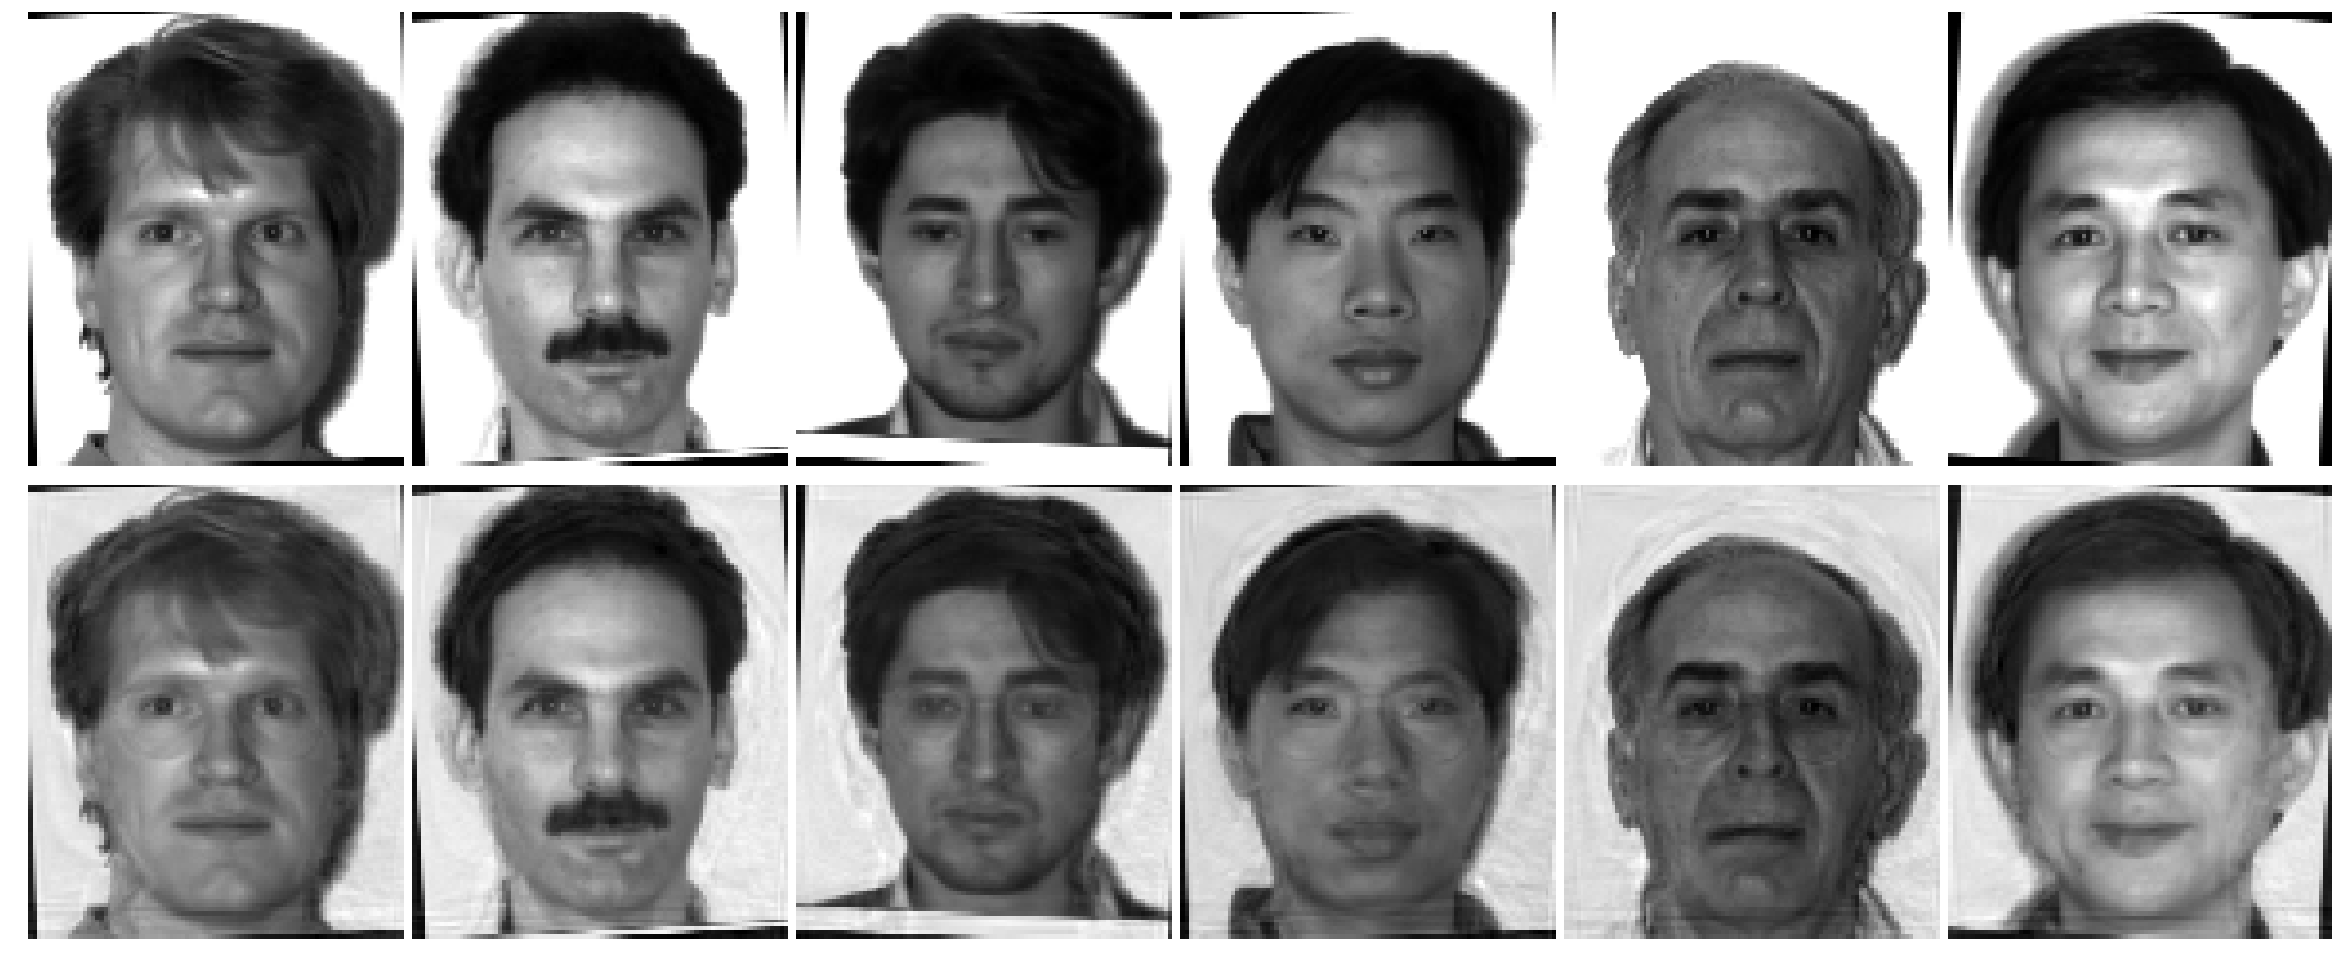
\includegraphics[width = \textwidth]{Chapters/07_DimemsionalityReduction/28_pca2/latex/yaleb_ori_res.pdf}
    \caption[]{Hàng trên: các ảnh gốc. Hàng dưới: các ảnh được \textit{suy ra} từ eigenfaces. Ảnh ở hàng dưới có nhiều nhiễu nhưng vẫn mang những đặc điểm riêng mà mắt người có thể phân biệt được.}
    \label{fig:28_3}
\end{figure}
Như vậy, vector với số chiều $K = 100$ trong không gian mới mang \textit{khá} đầy đủ thông tin của vector có số chiều $D = 11368$ trong không gian ban đầu. 
 
Phần còn lại của source code có thể được tìm thấy \href{https://github.com/tiepvupsu/tiepvupsu.github.io/blob/master/assets/28_pca2/python/EigenFaces.ipynb}{tại đây}. 
 
 
\subsection{Unsupervised Abnormal Detection}
Ngoài các ứng dụng về nén và classification, PCA còn được sử dụng trong nhiều lĩnh vực khác nhau. Abnormal Detection (dò tìm các hiện tượng không bình thường) là một trong số đó. Thêm nữa, giả sử chúng ta không biết nhãn của các sự kiện này, tức ta đang làm việc với một bài toán Unsupervised. 
 
 Ý tưởng cơ bản là các sự kiện 'normal' thường nằm gần một không gian con nào đó, trong khi các sự kiện 'abnormal' thường khác biệt với các sự kiện 'normal', tức nằm xa không gian con đó. Hơn nữa, vì là 'abnormal' nên số lượng các sự kiện thuộc loại này là rất nhỏ so với 'normal'. 
 
Như vậy, chúng ta có thể làm PCA trên toàn bộ dữ liệu để tìm ra các thành phần chính của dữ liệu, từ đó suy ra không gian con mà các điểm 'normal' nằm gần. Việc xác định một điểm là 'normal' hay 'abnoral' được xác định bằng cách đo khoảng cách từ điểm đó tới không gian con tìm được. 
 
Hình 4 dưới đây minh hoạ cho việc xác định các sự kiện không bình thường. 
 
% <hr> 
% <div> 
% <table width = "100%" style = "border: 0px solid white"> 
 
%     <tr > 
%         <td width="40%" style = "border: 0px solid white" align = "center"> 
%         <img style="display:block;" width = "100%" src = "/assets/28_pca2/abnormal.png"> 
%          </td> 
%         <td width="40%" style = "border: 0px solid white" align = "justify"> 
%         Hình 4: PCA cho việc xác định các sự kiện 'abnormal' với giả sử rằng các sự kiện 'normal' chiếm đa số và nằm gần trong một không gian con nào đó. Khi đó, nếu làm PCA trên toàn bộ dữ liệu, không gian con thu được gần với không gian con của tập các sự kiện 'normal'. Lúc này, các điểm quá xa không gian con này, trong trường hợp này là các điểm màu cam, có thể được coi là các sự kiện 'abnormal'. 
%         </td> 
%     </tr> 
% </table> 
% </div> 
% <hr> 

\begin{figure}[t]
    % caption on side     
    \floatbox[{\capbeside\thisfloatsetup{capbesideposition={right,top},capbesidewidth=6cm}}]{figure}[\FBwidth]
    {\caption{ 
    PCA cho việc xác định các sự kiện 'abnormal' với giả sử rằng các sự kiện 'normal' chiếm đa số và nằm gần trong một không gian con nào đó. Khi đó, nếu làm PCA trên toàn bộ dữ liệu, không gian con thu được gần với không gian con của tập các sự kiện 'normal'. Lúc này, các điểm quá xa không gian con này, trong trường hợp này là các điểm màu cam, có thể được coi là các sự kiện 'abnormal'.
    }
    \label{fig:28_4}}
    { % figure here
    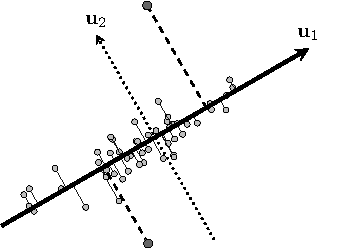
\includegraphics[width=.5\textwidth]{Chapters/07_DimemsionalityReduction/28_pca2/latex/abnormal.pdf}
    }
\end{figure}

 
Một ứng dụng của việc này có thể được tìm thấy trong bài báo: \href{http://www.cs.bu.edu/fac/crovella/paper-archive/sigc04-network-wide-anomalies.pdf}{Diagnosing Network-Wide Traffic Anomalies}. 
 
 
\section{Thảo luận}
\begin{itemize}
\item PCA là một phương pháp Unsupervised. Việc thực hiện PCA trên toàn bộ dữ liệu không phụ thuộc vào class(nếu có) của mỗi dữ liệu. Việc này đôi khi khiến cho PCA không mang lại hiệu quả cho các bài toán classification. Thật vậy, giả sử trong không gian hai chiều, 2 classes phân bố dọc hai bên của 1 đường thẳng. Như vậy, PCA nhiều khả năng sẽ cho chúng ta giữ lại thành phần chính chính là đường thẳng đó. Khi chiếu dữ liệu lên đường thẳng này, cả hai classes bị trộn lẫn vào nhau, khiến cho việc classification đạt kết quả thấp. Có một phương pháp tương tự như PCA giúp tận dụng thông tin về các class để xác định chiếu theo chiều nào, phương pháp đó có tên là \href{https://en.wikipedia.org/wiki/Linear_discriminant_analysis}{Linear Discriminant Analysis}, sẽ được thảo luận trong bài tiếp theo. 
 
\item Với các bài toán Large-scale, đôi khi việc tính toán trên toàn bộ dữ liệu là không khả thi vì còn có vấn đề về bộ nhớ. Giải pháp là thực hiện PCA lần đầu trên một tập con dữ liệu vừa với bộ nhớ, sau đó lấy một tập con khác để (incrementally) cập nhật nghiệm của PCA tới khi nào hội tụ. Ý tưởng này khá giống với \href{http://machinelearningcoban.com/2017/01/16/gradientdescent2/#-mini-batch-gradient-descent}{Mini-batch Gradient Descent}, và được gọi là \href{http://cseweb.ucsd.edu/~dasgupta/papers/incremental-pca.pdf}{Incremental PCA}. 
 
\item Ngoài ra, còn rất nhiều hướng mở rộng của PCA, bạn đọc có thể tìm kiếm theo từ khoá: Sparse PCA, Kernel PCA, Robust PCA. 
\end{itemize}
 
 
\section{Tài liệu tham khảo}
[1] \href{https://www.youtube.com/watch?v=F-nfsSq42ow}{PCA, SVD} 
 
[2] \href{https://en.wikipedia.org/wiki/Eigenface}{Eigenface} 
 
[3] \href{http://cseweb.ucsd.edu/~dasgupta/papers/incremental-pca.pdf}{The Fast Convergence of Incremental PCA} 
 
[4] \href{http://www.cs.bu.edu/fac/crovella/paper-archive/sigc04-network-wide-anomalies.pdf}{Diagnosing Network-Wide Traffic  Anomalies} 
 
